\documentclass{article}

\usepackage[a4paper, top=2cm, bottom=3cm]{geometry}
\usepackage{babel}[german]
\usepackage{booktabs}
\usepackage{mathtools}
\usepackage{amssymb}
\usepackage{enumitem}
\usepackage{amsmath}

\usepackage{hyperref}

\usepackage{graphicx}
\usepackage{wrapfig}
\usepackage{siunitx}

\newcommand{\proofeq}{\overset{!}{=}}
\newcommand{\proofeqv}{\overset{!}{\Leftrightarrow}}
\newcommand{\equivalent}{\overset{\scriptscriptstyle\wedge}{=}}
\DeclarePairedDelimiter\ceil{\lceil}{\rceil}
\DeclarePairedDelimiter\floor{\lfloor}{\rfloor}

\date{7.03.2022}
\title{Physikalisches Grundpraktikum Teil I \\ (Mechanik und Thermodynamik) \\ Versuch 6 Innendruck eines Luftballons}
\author{Finn Wagner}

\begin{document}
    \maketitle

    \section{Versuchsziel und Versuchsmethode}
    In diesem Versuch wird mit Hilfe der Ausströmgeschwindigkeit der Luft eines Luftballons über die Bernoulligleichung sein Innendruck bestimmt.
    Also der Druck, der durch die Dehnung des Gummis entsteht.

    \section{Grundlagen}
    Die Bernoulligleichung beschreibt Druck und Strömung von Gasen und Flüssigkeiten.
    \begin{equation} \label{eq:bernoulli}
        p + \rho g h + \frac{\rho}{2} v^2 = p_t = const
    \end{equation}
    Diese Form der Bernoulligleichung nennt man auch Druckgleichung.
    Sie setzt den totalen Druck \( p_t \) in Verbidung mit dem dynamische Druck \(p_{dyn} = \frac{\rho}{2} v^2\), 
    dem statischen Druck \( p \) und dem aus der Erdbeschleunigung entstehenden Druck \( \rho g h  \).
    Wichtig anzumerken ist hier, das die Bernoulligleichung eine ideale Strömung voraussetzt.
    Also dass das Fluid laminar fließend, es inkompressibel ist und es keine innere Viskosität besitzt 
    Außerdem muss die Dichte \( \rho \) des Fluids, sowie der Druck entlang aller möglichen Stromlinie konstant sein.
    Vereinfachend nehmen wir auch an, das die Geschwindigkeit entlang aller Stromlinien indentisch ist. TODO: Quelle Aufgabenstellung
    Außerdem wird die Reibung des Fluids an Oberflächen vernachlässigt.
    Für genauere Berechnung könnten Korrekturterme für Luft aus der Fachliteratur entnommen werden.

    In unserem Versuch verwenden wir einen aufgeblasenen Luftballon, aus welchem Luft (auf Grund von Druckdifferenzen) mit \(v_a\) ausströmt. 

    Für unseren Versuch spielt der Druck, der aus der Schwerkraft entsteht keine Rolle.
    Der Versuch kann mit dem Luftballon und Mundstück horizontal zum Boden (Siehe Abbildung\ref{fig:messungen}, a horizontal) durchgeführt werden.
    Damit spielt die Schwerkraft bei der Bewegung des Gases keine Rolle. Aber auch bei Messungen bei denen der Luftballon z.B. einfach losgelassen wird,
    ist der Effekt zu vernachlässigen.

    Beispielhaft berechnen wir den maximalen Druckbeitrag (hydrostatischer Druck (TODO: Quelle 7).
    Die Länge des Luftballons sei \(h = \SI{0.25}{m}\), die Dichte der Luft \(\rho = \SI{1.2041}{\frac{kg}{m^3}} \) TODO: Quelle 
    und die Erdbeschleunigung \(g = \SI{9.81}{\frac{m}{s^2}} \)
    \begin{equation}
        \SI{0.25}{m} \cdot \SI{1.2041}{\frac{kg}{m^3}} \cdot \SI{9.81}{\frac{m}{s^2}} = \SI{2.95}{Pa} % 0.25m * 1.20141kg/m^3 * 9.81m/s^2 as pascals
    \end{equation}
    Es ergeben sich \(\SI{2.95}{Pa}\) ein, wie wir später in der Auswertung sehen werden, vernachlässigbarer Beitrag.

    Wir wissen das der Innendruck des Luftballons \(p_i\) größer ist als der Außendruck \(p_a\)
    und sich nur um den dynamischen Anteil mit der Ausströmungsgeschwindigkeit \(v_a\) unterscheidet. Mit der Dichte des strömenden Mediums Luft \( \rho \) folgt: 
    \begin{equation} \label{eq:ballon_druck}
        p_i = p_a + \frac{1}{2} \rho v_a^2
    \end{equation}
    \begin{figure}[h]\label{fig:luftstoss}
        \centering
        \includegraphics[width=7cm]{luftstoß.png}
        \caption{Veranschaulichung des Versuchs und Gleichung\ref{eq:ballon_druck}}
    \end{figure}

    Weiterhin nehmen wir den Innendruck des Luftballons als während des Versuchs konstant an.
    Ziel des Versuches ist es die Druckdifferenz \( (p_i - p_a) := p_b \) also den Überdruck des Ballons (TODO: Quelle [9]) zu bestimmen.

    \section{Versuchsaufbau und Durchführung}
    
    \begin{figure}[h]\label{fig:messungen}
        \centering
        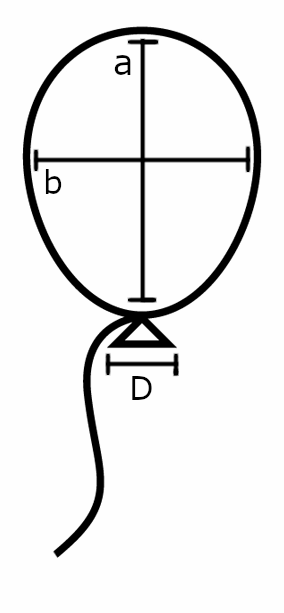
\includegraphics[height=6cm]{luftballons.png}
        \caption{Messgrößen am Luftballon}
    \end{figure}

    \subsection{Aufbau und Material}
    \begin{itemize}
        \item Maßband mit mindestens Milimetergenauigkeit, am besten ein weiches Rollbandmaß
        \item Stoppuhr (Genauigkeit mindestens \( \frac{1}{10}s \))
        \item Smartphone zur Videoaufnahme
    \end{itemize}

    \subsection{Durchführung}
    \begin{enumerate}
        \item Bestimmen sie den Durchmesser D des Mundstückes.
        \item Blasen sie den Luftballon auf. Halten sie das Ende zu. Bestimmen Sie den Umfang mithilfe des Maßband.
        Messen Sie den Umfang von Mundstück bis zum obersten Punkt (Umfang a), sowie den Umfang der "Tallie" (Umfang b).
        \item Lassen Sie die Luft aus dem Ballon ausströmen. Der Luftballon muss nicht festgehalten werden.
        Messen Sie die Zeit, in welcher die Luft aus dem Luftballon entweicht.
        Nutzen Sie die Stoppuhr oder werten sie die Zeit am Video aus. Für Videoaufnahmen empfielt es sich den Ballon festzukleben. TODO: Bild
        \item Wiederholen Sie die Messung (Schritt 2 \& 3) drei mal und notieren Sie ihre Ergebnisse.
    \end{enumerate}

    \section{Formeln}
    Die direkt gemessenen Größen sind der Umfang des Luftballons, die Ausströmzeit, sowie der Durchmesser des Mundstücks.
    Für unsere Auswertung brauchen wir die durchströmte Fläche des Mundstücks (Querschnittsfläche).
    Die Fläche also, durch die die Luft im Luftballon entweicht.
    Mit der Formel für die Fläche eines Kreises \( A = \pi {r}^2 \) und der Beziehung \( \frac{D}{2} = r\) folgt:
    \begin{equation} \label{eq:durch_flache}
        A = \pi {\left( \frac{D}{2} \right)}^2
    \end{equation}
    Weiterhin berechnen wir das Volumen \(V\) des Luftballons.
    Wir nähern den Luftballon als kugelsymmetrisch und vernachlässigen das Volumen des Mundstücks.
    Der Umfang \(U\) einer Kugel (2 Dimensionen) ist der eines Kreises mit \(U = 2 \pi r\). Umgeformt nach \(r\) ergibt sich \(\frac{U}{2 \pi} = r\).
    Wir berechnen den Durchschnitt der gemessenen Umfänge \(a\) und \(b\) um das Volumen besser als Kugel zu approximieren.
    Die Formel für das Volumen einer Kugel ist \( V = \frac{4}{3} \pi r^3 \).
    Um das Volumen aus dem Umfang zu berechnen setzen wir für den Radius ein:
    \begin{equation} \label{eq:volumen}
        V = \frac{4}{3} \pi {\left( \frac{U}{2 \pi} \right) }^3 = \frac{4}{3} \pi \frac{U^3}{8 \pi^3} = \frac{1}{6} \frac{U^3}{\pi^2}
    \end{equation}
    Im nächsten Schritt stellen wir die im Skript gegebene Gleichung nach \(v_a\) um.
    \[ V = A \cdot v_a \cdot t_a \Rightarrow v_a = \frac{V}{A \cdot t_a}\] TODO: Wo kommt die Formel her?
    Hier setzen wir nun die Formel für das Volumen(\ref{eq:volumen}) und die durchströmte Fläche (\ref{eq:durch_flache}) ein.
    \begin{equation} \label{eq:calc_velocity}
        v_a = \frac{V}{A \cdot t_a} = \frac{\frac{1}{6} \frac{U^3}{\pi^2} }{ \pi {\left(\frac{D}{2}\right)}^2 \cdot t_a} = \frac{2}{3} \frac{U^3}{\pi^3 D^2 t_a}
    \end{equation}
    Umstellungsprobe durch Einheitenrechnung: \\
    \begin{equation*}
        \frac{m^3}{m^3 \cdot s} = \frac{m}{s}
    \end{equation*}  


    \section{Auswertung}
    Wir berechnen aus den drei Versuchen jeweils die Ausströmgeschwindigkeiten \(v_1\) bis \(v_3\). \\
    Zuerst berechnen wir den Innendurchmesser des Mundstücks aus den drei gemessenen Werten TODO: Ref Messwerte
    \(\SI{1.15}{cm}, \SI{1.1}{cm}, \SI{1.2}{cm} \). Das ergibt
    \begin{equation}
        \frac{ (\SI{1.15}{cm} + \SI{1.1}{cm} + \SI{1.2}{cm}) }{3} = \SI{1.15}{cm} = \SI{0.0115}{m}
    \end{equation}
    Die Fläche \(A\) des Mundstücks beträgt \( \pi {\left( \frac{ \SI{0.0115}{m} }{2} \right)}^2 = 1.03869 \cdot 10^{-4} \si{m^2} \).

    \subsection{Durchführungen}
    Für alle Durchführungen wurde ein Wert für \(a\) und ein Wert für \(b\) gemessen, sowie 2 bis 3 Zeitmessungen.
    Aus \(a\) und \(b\) wird der Durchschnitt \(U\) als Umfang verwendet.
    Als Zeit \(t_a\) wurde ebenso der Durchschnitt der gemesenen Ausströmzeiten verwendet.

    \subsubsection{Durchführung 1}
        Luftballonumfang: \(a = \SI{0.584}{m}, b = \SI{0.511}{m} \). Durchschnitt: \(U = 0.5475m\) \\
        Ausströmzeit \( \frac{\SI{1.34}{s} + \SI{1.04}{s} }{2} = 1.19s \) \\
        Einsetzen der Werte in die Formel (\ref{eq:calc_velocity}): \\
        \[ v_a = \frac{2}{3} \frac{{(0.5475m)}^3}{\pi^3 {(0.0115m )}^2 \cdot 1.19s} = 22.42 \frac{m}{s} \]
        % 2/3 * U^3 /(pi^3 D^2 t) where U = 0.5475, D=0.0115, t =1.19

    \subsubsection{Durchführung 2}
    TODO: Durchführung 2 Machen

    \(a = 0.615 m\) \(b = 0.564 m\) Durchschnitt der Luftballonumfänge \(U = 0.5895m\) \\
    Die beiden durchgeführten Zeitmessungen weichen stark voneinander ab: \\
    \( (1.45s + 1.61s + 1.64s )/3 = 1,5\bar{6}s \) \\
    Wir setzen in die oben berechnete Formel ein: \\
    \[ v_a = \frac{2}{3} \frac{{(0.5895m)}^3}{\pi^3 {(0.0115m )}^2 \cdot 1,5\bar{6}s} = 21,25877656 \frac{m}{s} \]

    \subsection{Mittlere Geschwindigkeit}
    \( 22.4217162 \frac{m}{s}, 24.8927916 \frac{m}{s}, 21,25877656 \frac{m}{s} \) \\
    Wir berechnen den Mittelwert der Ausströmgeschwindigkeiten: \\
    \( ( 22.4217162 \frac{m}{s} + 24.8927916 \frac{m}{s} + 21,25877656 \frac{m}{s} )/3 = 22.85776145 \frac{m}{s} \) \\
    -umrechnen mit Bernoulligleichung

    \subsection{Umrechnen zum Überdruck}
    Die Bernoulligleichung verbindet Drücke und Strömungsgeschwindigkeiten. 
    Wobei \(p_i\) der Innendruck des Luftballons und \(p_a\) der Außen/Umgebungsdruck\\
    \(p_i = p_a + \frac{1}{2} \rho v_a^2\)
    \(p_i - p_a\) ist die Druckdifferenz zwischen dem Inneren und Äußeren des Ballons. Also \\
    \( (p_i - p_a) = \frac{1}{2} \rho v_a^2 \) \\
    Gegeben in Aufgabe für \( P_a = 101 325 Pa\) und \(\rho = 1.2041 \frac{kg}{m^3} \) bei 20° Celsius auf Meereshöhe \\
    Eingesetzt
    \[ (p_i - p_a) = \frac{1}{2} \cdot 1.2041 \frac{kg}{m^3} \cdot {(22.85776145 \frac{m}{s})}^2 = 314.557 Pa \]
    
    \subsection{Versuch mit verkleinerter Öffnung}
    TODO: ?

    \subsection{Weltall}
    Umformungen
    FAKTOR!!!

    \section{Fehlerrechnung}
        \subsection{Messunsicherheit}
            Wir bestimmen zunächst die Messunsicherheiten für den Versuch.
            Direkt gemessen wurde der Umfang, daraus ergibt sich die Messunsicherheit \(\Delta U\)
            und die Zeit für das entweichen der Luft, hier die Messunsicherheit \(\Delta s\)

            Die Längenmessungen wurden mit einenm handelsüblichen Maßband mit einer Genauigkeit von 1mm gemacht.
            Die Unsicherheit \( \Delta U \) könnte man naiv als \( \approx \SI{0.1}{cm} \) annehmen, aus der Genauigkeit des Maßbandes.
            Beim Durchführen des Versuches wird jedoch schnell klar, dass es gar nicht so einfach ist ein Maßband an einen Ballon anzulegen.
            Das Maßband kann seitlich verrutschen und so den gemessenen Weg vergrößern oder man zieht zu stark und drückt den Ballon ein.
            Um den Messfehler für die Umfangsmessung besser abschätzen zu können wurden
            6 weitere Messungen bei einem aufgepusteten Ballon gemacht.
            Es wurde wiederholt der gleiche Umfang gemessen, um abschätzen zu können um wie viel die Werte von einander abweichen.
            Die Standardabweichung der 6 Messungen beträgt \( \approx \SI{0.9}{cm}\)\ref{Messfehler_Umfang} und wird hier als Abweichung angesetzt.
            
            Die Auflösung der für den Versuch verwendeten Stoppuhr (Handystoppuhr) ist eine \(\SI{1}{ms}\).
            Die menschliche Reaktionszeit beträgt aber bereits \(\approx \SI{180}{ms} \) TODO:LINK
            Um den abklingenden Ton oder den sich nicht mehr veränderden Ballon zu reagieren verstreicht also bereits eine ganze Weile.
            Bis dann die Stoppuhr gedrückt wurde sind dann bereits \(\approx \SI{0.2}{s}\) vergangen.
            Da die gleiche Verzögerung auch beim Beginn der Messung entsteht schätzen wir den Messfehler auf \(\SI{0.25}{s}\)
            Nicht einfach zu beurteilen, ist auch wann der Ballon wirklich ``leer´´ ist. TODO: Mehr
            Bei unseren Durchführungen stoppten mehrere Personen gleichzeitig nach einem Countdown die Zeit. Die Messungen der
            Person die den Ballon selber losließ war \(\approx \SI{0.2}{s} \) länger als die der anderen Messenden.
            Was sich ebenfalls auf die Reaktionszeit zurückführen lässt.
            TODO: Video aufgenommen ausgewertet mit Media Player Classic ausgewertet
            TODO: Beachten Vidoe nur mit 30fps aufgenommen Fehlerrechnung

            Nach eingien weiteren Experimenten mit dem Luftballon zeigte sich außerdem das die Spannkraft nachließ und das Volumen
            nicht zu seiner Ausgangsgröße zurückkehrte, sich also der Innendruck des Luftballons änderte.
            Die hier verwendeten Messungen fanden am selben Ballon, mit den ersten drei Aufpustvorgängen statt, womit der Effekt noch vernachlässigbar ist.

            Die durchströmte Fläche A wird als fehlerlos angenommen.

        \subsection{Fehlerforpflanzung}
            Den Fehler für die berechnete Geschwindigkeit bekommen wir mithilfe der Gaußschen Fehlerfortpflanzung (0.2.1.14 aus TODO:Link[4])
            Wir setzen die Funktion zur Berechnung von \(v_a\)\ref{eq:calc_velocity} durch die beiden (fehlerbehafteten, D ist fehlerlos)
            direktgemessenen Größen, in die Fehlerfortplanzungsformel ein und berechnen den Messfehler für die Ausströmgeschwindigkeit. 
            \begin{equation}
                \Delta v_a = \sqrt{ {\left( \frac{ \partial v_a }{ \partial t_a } \cdot \Delta t \right)}^2 + {\left( \frac{ \partial v_a }{ \partial U } \cdot \Delta U \right)}^2 }
            \end{equation}
            Wir berechnen die in der Formel benötigten partiellen Ableitungen:
            \begin{equation}
                 \frac{\partial v_a}{ \partial t_a} = \frac{2}{3} \frac{U^3}{\pi^3 D^2} \frac{-1}{t_a^2}
            \end{equation}
            \begin{equation}
                \frac{\partial v_a}{ \partial U} = \frac{2}{3} \frac{1}{\pi^3 D^2 t_a} 2 U^2
            \end{equation}
            Einsetzen:
            \begin{equation}
                \Delta v_a = \sqrt{ {\left( \frac{2}{3} \frac{U^3}{\pi^3 D^2} \frac{-1}{t_a^2} \cdot \Delta t \right) }^2 
                + {\left( \frac{2}{3} \frac{1}{\pi^3 D^2 t_a} 3 U^2 \cdot \Delta U \right)}^2 }
            \end{equation}
            Vereinfachen:
            \begin{equation}
                \Delta v_a = \sqrt{ \frac{4}{9} \frac{ {(\Delta t)}^2 U^6}{\pi^6 D^4 t_a^4} + 4 \frac{U^4 {(\Delta U)}^2}{\pi^6 D^4 t_a^2}}
            \end{equation}

        \subsection{Fehler Durchführung 1}
            \[ \Delta v_a = \sqrt{ \frac{4}{9} \frac{ {(\Delta t)}^2 U^6}{\pi^6 D^4 t_a^4} + 4 \frac{U^4 {(\Delta U)}^2}{\pi^6 D^4 t_a^2}} \]
            % sqrt((4 b^2 U^4)/(D^4 π^6 t^2) + (4 a^2 U^6)/(9 D^4 π^6 t^4)) with U = 0.5474, D=0.0115, t=1.19, a=0.25, b=0.005
            Wären 4.74 m/s Abweichung :()

        \subsection{Fehler mittlere Geschwindigkeit}
        \subsection{Fehler umrechnen auf Überdruck}
    
    \section{Ergebnis}
        Hier die korrigierten Werte?
        TODO: Kommastellen wegmachen \\

    \section{Diskussion}
        Ergebnis gut für Größenordnung sonst nichts, nicht veralgemeinerbar auf verschiedene Luftballons, Größe, Spannkraft etc.

        Den Fehler, der entsteht, da das Mundstück nicht Teil des Luftballonvolumens ist und der Luftballon keine Kugel ist wird hier nicht berücksichtigt.
        Hätte aber einen erheblichen Einfluss auf die Ungenauigkeit. Sehr schwache Annahme.
        TODO: Abhängig von Ballonbeschaffenheit \\
        TODO: Abhägig wie doll aufgepustet? Weggemittelt \\
        TODO: Bernoullifehler Luft 2.95Pa

    TODO: FOTOS !!!
    \section{Quellen}
    % [1] \url{https://de.wikipedia.org/wiki/Bernoulli-Gleichung#Druckgleichung} \\
    % [2] Experimentalphysik I: Mechanik und Elemente der Wärmelehre; Vorlesung von Sangam Chaterjee \\
    % [3] \url{https://www.schule-und-familie.de/malvorlagen/karneval-fasching-fastnacht/luftballons.html}, bearbeitet mit Anmerkungen \\
    % [4] Anleitung zum Physikalischen Grundpraktikum Teil I (Mechanik und Thermodynamik) JLU Gießen II. Physikalisches Institut Version 1.3, 28.02.2022 von Jens Sören Lange
    % [5] https://www.bussgeldkatalog.org/reaktionszeit/#
    % [6] https://www.studienkreis.de/mathematik/varianz-standardabweichung/
    % [7] https://www.lexas.de/klima/klimaelemente/luft/luftdruck.aspx
    % [8] https://de.dreamstime.com/e-r-image147149352
    % [9] https://www.chemie.de/lexikon/%C3%9Cberdruck.html

    \section{Messfehler Abschätzung}\label{Messfehler_Umfang}
        Wir führen einen weiteren kleinen Versuch duch um die Messungenauigkeit des Umfangs bei einem Luftballon zu bestimmen.
        Dazu messen wir wiederholt den Umfang und untersuchen wie weit die Werte voneinander abweichen.
        TODO:Weg? Der Versuch wird an einem zugeknoteten Ballon durchgeführt, der sich deutlich leichter handhaben lässt als ein zugehaltener.
        Es wurde versucht diesen 
        \subsection{Durchführung}
            \begin{enumerate}
                \item Luftballon aufpusten und zuknoten.
                \item Mit Messmethode nach Wahl den Umfang (hier Umfang a) des Luftballons wiederholt messen.
            \end{enumerate}
        \subsection{Auswertung}
            Der Umfang a des Luftballons wurde 6 mal gemessen.
            \begin{center}
                \begin{tabular}{c c c c c c c}
                    Messung & 1 & 2 & 3 & 4 & 5 & 6 \\
                    \midrule
                    Messwert & 71.5cm & 69cm & 71.25cm & 71.7cm & 71.2cm & 71.6cm \\
                    
                \end{tabular}    
            \end{center}
        Wir berechnen den Druchschnitt der Messwerte:
        \[ d = \frac{ \SI{71.5}{cm} + \SI{69}{cm} + \SI{71.5}{cm} + \SI{71.7}{cm} + \SI{71.2}{cm} + \SI{71.6}{cm} }{ 6 }  = 71.04cm\]
        Die Varianz:
        \begin{gather*}
            V = \frac{1}{6} ( {( \SI{71.5}{cm} - \SI{71.04}{cm} )}^2 + {( \SI{69}{cm} - \SI{71.04}{cm} )}^2 + {( \SI{71.25}{cm} - \SI{71.04}{cm} )}^2 \\
               + {( \SI{71.7}{cm} - \SI{71.04}{cm} )}^2 + {( \SI{71.2}{cm} - \SI{71.04}{cm} )}^2 + {( \SI{71.6}{cm} - \SI{71.04}{cm} )}^2 )
             = \SI{0.86535}{{cm}^2}
        \end{gather*} 
        % ( (71.5-71.04)^2  + (69-71.04)^2  + (71.25-71.04)^2  + (71.7-71.04)^2  + (71.2-71.04)^2  +(71.6-71.04)^2  )/6
        Und zuletzt die Standardabweichung:
        \[ \sigma = \sqrt{\SI{0.86535}{{cm}^2}}  = \SI{0.90242}{cm} \]
        Die Messungen lagen im Abstand von ca. \(\SI{0.9}{cm}\) vom Mittelwert.
        Es ist also begründet anzunehmen, dass die Messunsicherheit ungefähr bei \(\SI{0.9}{cm}\) liegt.
        TODO: Quelle[6]

    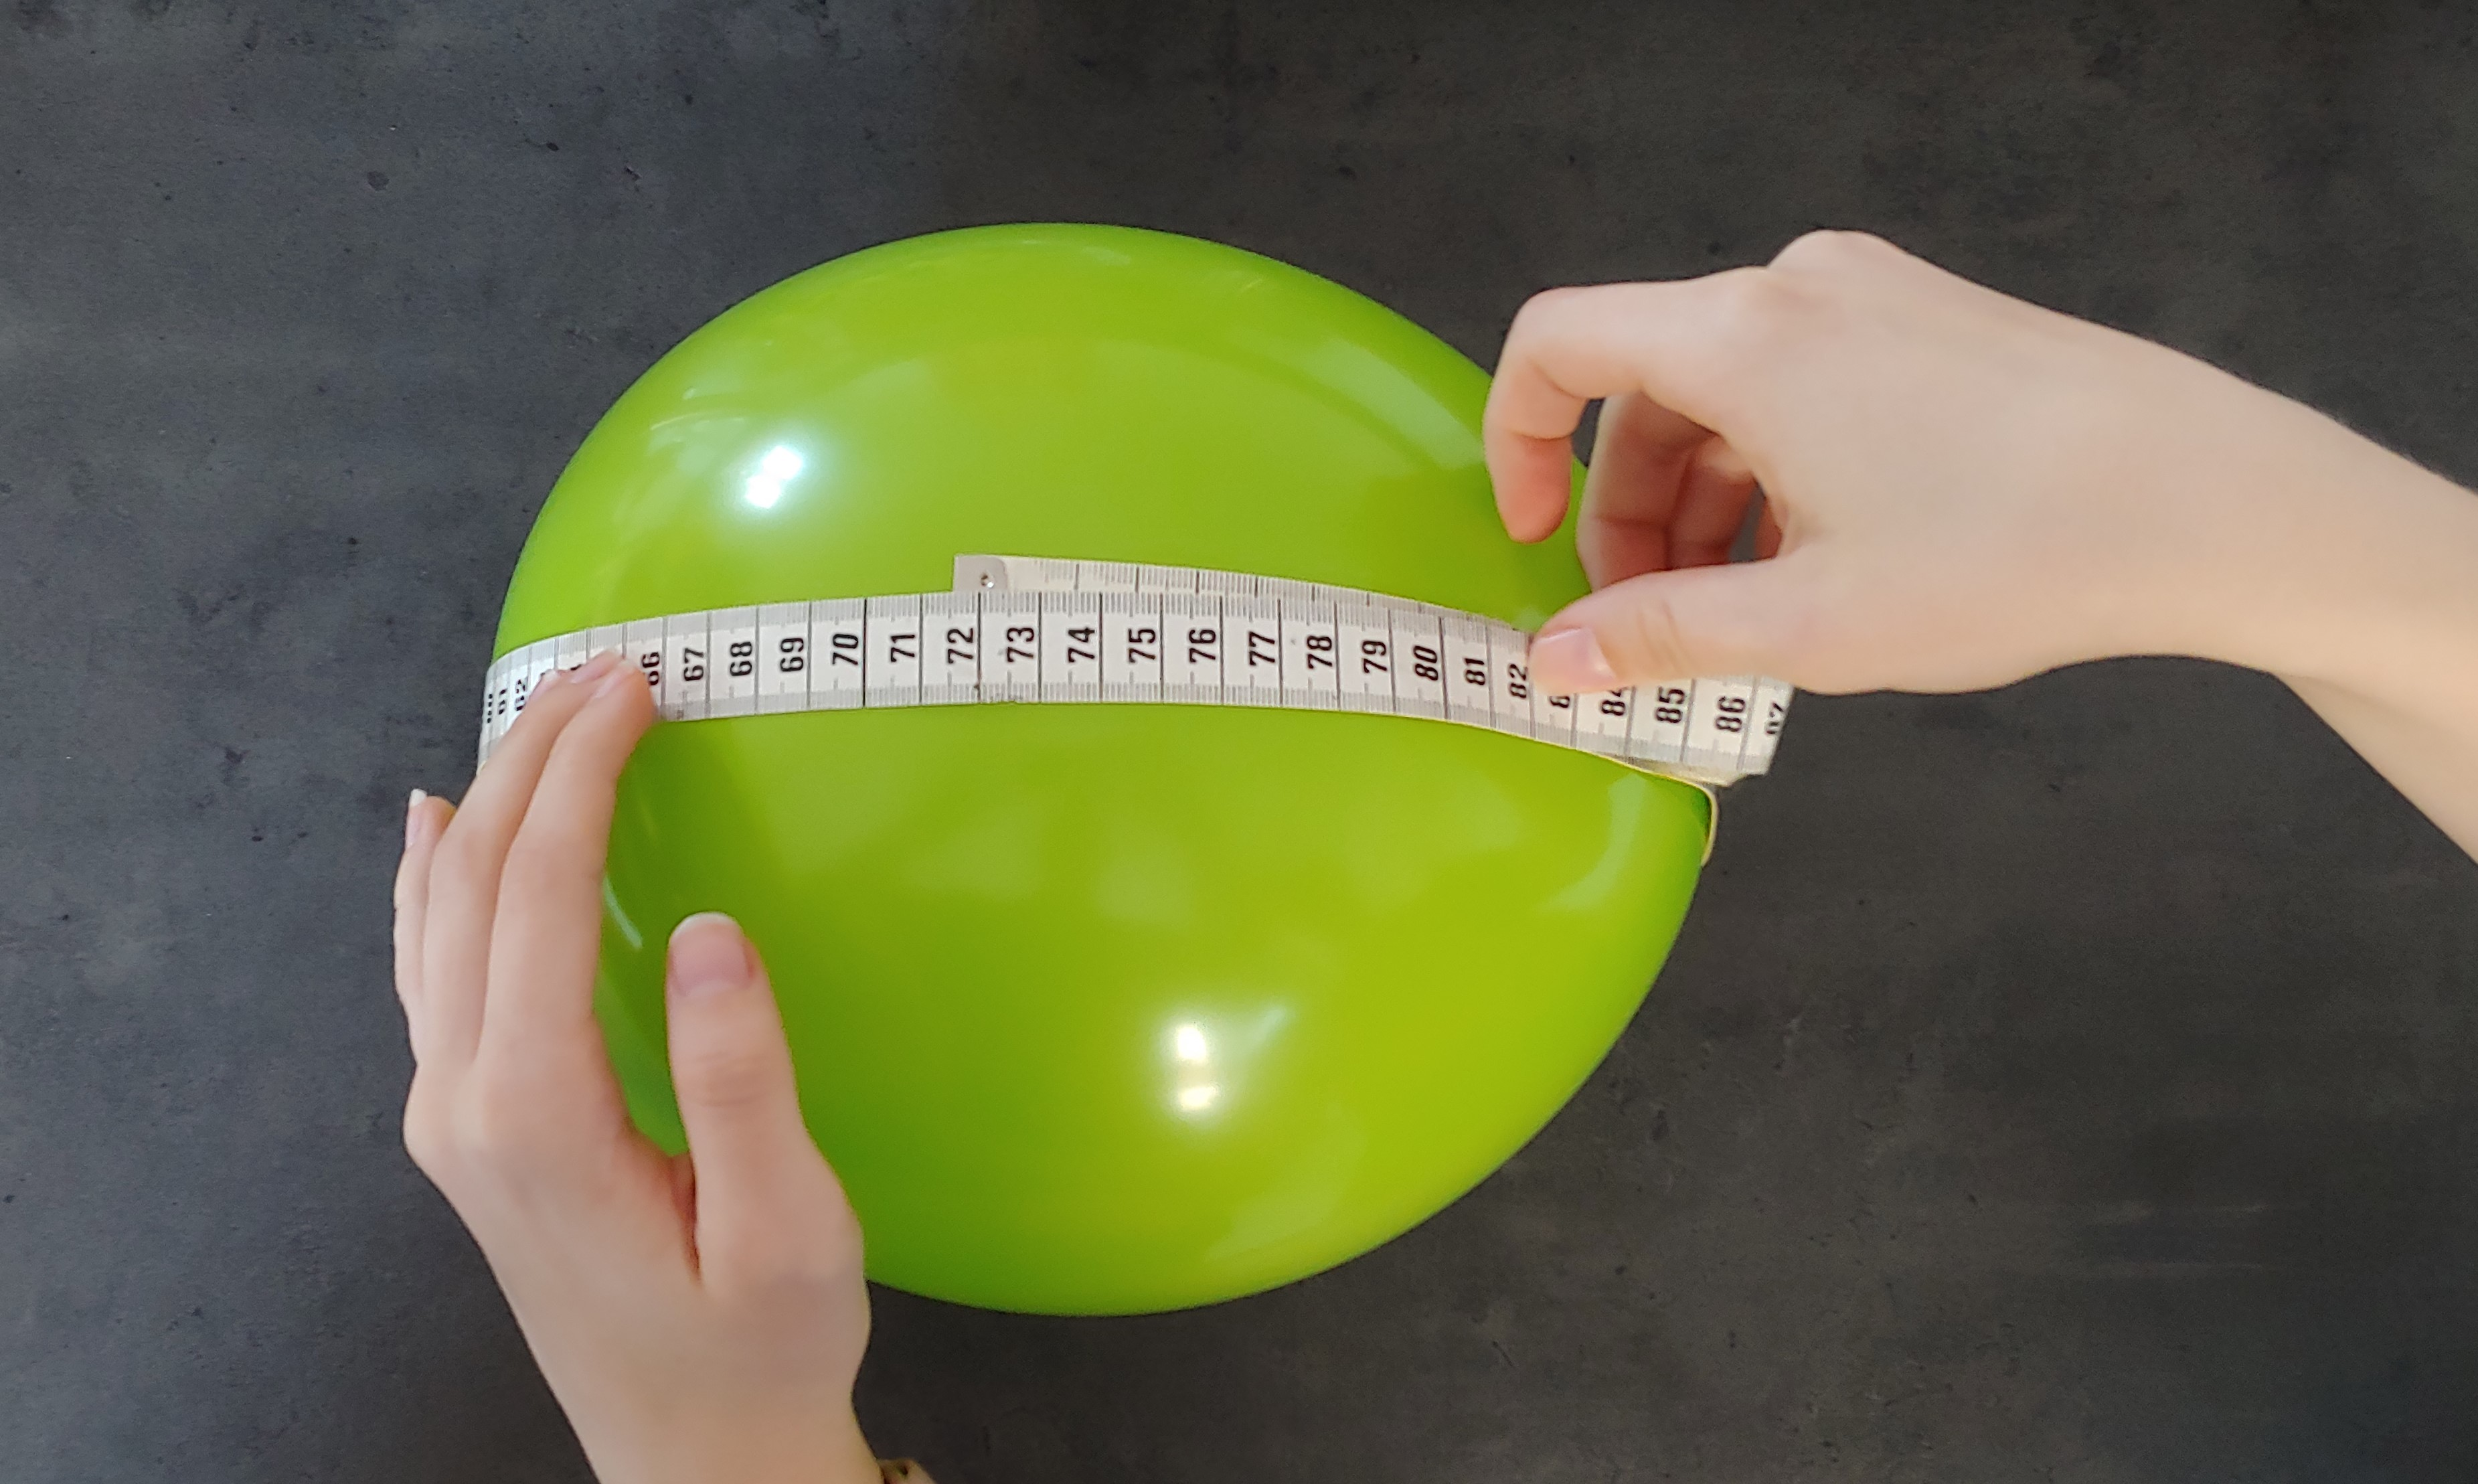
\includegraphics[scale=0.1]{luftballon_umfang_messung.jpg} % TODO: Bildunterschrift mit \section

\end{document}